\section{Choix de l'ordonnanceur}

	\subsection{Enjeux du choix de l'ordonnanceur}

	L'état de l'art nous a montré un vaste choix d'algorithmes qui présentent 
	des intérêts différents, et pour un certain nombre, 
	n'ayant pas pas encore été implémentés. \newline
	
	La première étape du travail consiste donc à départager ces algorithmes pour arrêter notre choix sur l'un d'entre eux. Ceci nécessite de clarifier nos attentes concernant le choix de l'ordonnanceur.\newline
	
	Pour rappel, les objectifs de ce travail sont de procéder à une implémentation dans 
	un \textbf{RTOS} dans plusieurs buts. 
	D'abord, en implémentant un algorithme qui n'a pas d'implémentation connue, nous 
	pouvons vérifier que ce passage de la théorie à la pratique est possible (car cela n'est pas 
	toujours évident), nous pouvons également mesurer ses performances. 
	Plus largement, nous pouvons émettre des propositions à l'attention de chercheurs 
	afin qu'ils puissent envisager de développer certains points lorsqu'ils proposent de nouveaux algorithmes. \newline
	
	Il est donc primordial de se tourner vers un algorithme qui pourra apporter sur le plan de 
	l'expérience des analyses intéressantes, c'est à dire exploitables pour la communauté. 
	Insistons peut-être sur le fait que des résultats ne sont pas nécessairement chiffrés mais 
	peuvent être des constats qualitatifs quant à la mise en œuvre elle-même.\newline
	
	\subsection{Pourquoi UEDF}
	
	Le choix le plus rationnel vis à vis des objectifs devrait se faire en fonction des 
	promesses théoriques de performance et de stabilité. 
	En effet, pour faire avancer la connaissance et permettre d'augmenter la confiance des utilisateurs 
	potentiels, il est judicieux de choisir un algorithme dont on attend au moins ceci :
	\begin{itemize}
		\item Un algorithme global
		\item Qui minimise le nombre de migrations
		\item L'ordonnanceur est en ligne, optimal pour la classe périodique
		\item Il n'a pas bénéficié d'une implémentation sur un \textbf{RTOS}
		\item Il promet des performances intéressantes
	\end{itemize}
	
	Le premier choix a été \hyperref[RUN]{RUN}[\ref*{RUN}], puis finalement, son descendant, \hyperref[QPS]{QPS}[\ref*{QPS}]. Ces choix étant guidés 
	sur leur intérêt d'ordonnanceurs en tant que tels.
	Toutefois, l'aspect très théorique des papiers les présentant a rendu la première phase de travail difficile. 
	En outre, nous n'avons pas trouvé d'implémentation ou de simulation malgré nos recherches.
	Finalement, nous n'avons pas réussi à entrer en contact avec les créateurs de ces algorithmes. \newline
	
	En effet, la possibilité de contacter les créateurs d'un algorithme peut singulièrement améliorer le 
	travail. Cela étant, cette nécessité découle du caractère très théorique de la littérature disponible
	et du manque fréquent de prise en considération des contraintes pratiques d'implémentation. 
	Pour illustrer cette remarque, un exemple assez commun est la non prise en considération 
	du fait que le fonctionnement des ordinateurs est évidemment discret, là où les 
	calculs présentés se basent sur un fonctionnement continu.
	Toute mise en pratique nécessite de faire des arrondis, ceux-ci doivent être cohérents.\newline

\todo{ajouter surcout dans le glossaire}
	Nous pouvons aussi évoquer les moments où l'algorithme doit faire des calculs. 
	Dans un simulateur, ou dans une vision idéalisée de l'ordonnanceur, l'on peut arrêter l'exécution 
	quand on le veut, avec des temps de surcoût [\ref*{surcout}]négligeables. Dans la réalité, comme on le verra, cela 
	n'est pas le cas. 
	Les auteurs qui connaissent bien ce fonctionnement auront la possibilité de devancer certaines questions.
	Néanmoins, dans le cas d'un papier très théorique qui s'emploie à faire des démonstrations mathématiques, 
	cela n'apparaîtra pas forcément.\newline
	
	\textbf{UEDF} bénéficie quant à lui d'une littérature qui développe mieux l'aspect pratique, et cela a orienté notre choix.\newline
	
	\todo{déplacer ça ailleurs}
	De plus, il y a des difficultés particulières liées au fait qu'un ordonnanceur ne soit qu'une partie d'un ensemble : 
	un \textbf{RTOS}. En effet, l'ordonnanceur n'est qu'une partie du kernel, et dépend de l'implémentation 
	d'autres parties du kernel, comme du dispatcher. Le travail d'implémentation d'un ordonnanceur ne consiste 
	pas à modifier tout le RTOS, mais à ajouter une partie du kernel. On ne peut 
	pas considérer l'ordonnanceur comme une tâche indépendante du reste du kernel, cela 
	implique un certain nombre de contraintes et de difficultés.\newline
	
	En d'autres termes, l'implémentation d'un ordonnanceur peut s'avérer une tâche bien compliquée selon que l'auteur du papier décrivant l'algorithme 
	ait une bonne connaissance des \textbf{RTOS} ou pas. 
	\newline

	
	Finalement, c'est un argument quant à la communication (clarté, possibilité de poser des questions) 
	qui a fixé le choix. Par conséquent, c'est \textbf{UEDF} qui a été sélectionné, car 
	non seulement il respectait 
	les promesses énoncées auparavant, mais aussi, en plus d'être très bien documenté, 
	nous pouvions poser nos questions directement à l'un de ses créateurs. Néanmoins, ses paramètres sont moins idéaux, 
	et nous avons revu nos attentes quant à l'efficacité à la baisse. Cela n'a en rien 
	modifié l'objet scientifique, à savoir le regard critique et la proposition d'améliorations 
	afin de stimuler et faciliter des implémentations futures, mais cela a sans doute 
	diminué les performances finales obtenues, tel que nous le verrons dans la partie Résultats.\newline
	
	
	\subsection{Présentation UEDF}
	
	Nous avons déjà présenté précédemment \textbf{UEDF}, de façon globale et succincte. 
	Dans cette partie, nous allons détailler \textbf{UEDF} afin d'en avoir une meilleure compréhension. Cela 
	permettra de mesurer la différence entre les attentes théoriques et les résultats obtenus.\newline

	Nous avons évoqué les intérêts de l'implémentation d'\textbf{UEDF} :\\
	Tout d'abord, il est principalement \hyperref[inline]{en ligne}, ce qui n'est pas le cas de 
	la plupart des ordonnanceurs utilisés dans l'industrie.
	Ensuite, il est global. Or, la plupart des ordonnanceurs 
	globaux connus et implémentés ne sont pas optimaux (pour la classe périodique), pour la
	raison exposée au préalable dans ce travail : il est nécessaire d'avoir de la clairvoyance, 
	c'est à dire une connaissance relative du futur.\newline
	
	Pour analyser son fonctionnement, nous devons poser quelques définitions. Aussi, par souci de clarté, nous posons que 
	l'offset [\ref*{offset}] de la tâche est nul dans la partie qui suit.\\
	\paragraph{Tâche active}\label{tacheactive}
	Ce qui définit une tâche "active" peut différer selon le contexte. Dans l'approche d'\textbf{UEDF}, une tâche est 
	considérée comme active si un travail a été relâché et que ce travail n'a pas encore atteint son échéance. 
	Un travail $\tau_i$ est actif s'il a été relâché sur ou après $t$ et que $d_i(t) > t$.
	Une tâche peut donc 
	être considérée comme active même si l'exécution d'un travail en cours est terminée. 
	Concrètement, si une tâche est périodique à échéance implicite [\ref*{echeancesurrequete}], elle est active en permanence dès le 
	premier relâchement de travail. Le travail sera actif durant son relâchement jusqu'à ce que $t >= d_i(t)$, où 
	une nouvelle instance de la tâche $\tau_i$ sera relâchée.
	
	
	\paragraph{Ensemble des tâches actives}\label{ensembledestachesactives}
	Dans \textbf{UEDF}, on effectue le parcours d'une liste des tâches actuellement actives dans le système, 
	cette liste étant ordonnée par échéances. 
	 L'ensemble des tâches actives est écrit $A(t)$ dans les formules qui suivent.\newline
	
	Pour décrire \textbf{UEDF}, nous allons le décomposer en étapes.
	À chaque fois qu'un nouveau travail est relâché, cela va provoquer le calcul suivant :\newline
	\paragraph{Allot}
	Les tâches actives [\ref*{tacheactive}] sont ordonnées dans une liste. La priorité est définie selon l'échéance, 
	la plus petite étant la plus prioritaire, comme dans \textbf{EDF} [\ref*{EDF}].
	Dans cette phase, l'algorithme va "réserver" des tranches de temps d'exécution des tâches sur les 
	processeurs, cela en calculant une valeur : \\
	$allot_{ij}$ pour $i \in \{0, nb\_de\_taches - 1\}$, pour $j \in \{0, nb\_processeurs - 1\}$
	La valeur $allot_{ij}$ représente le nombre d'unités d'exécution de la tâche $i$ réservé sur le processeur $j$.\newline
	Si cette valeur est positive, alors le temps $allot_{ij}$ du travail $i$ est réservé sur le 
	processeur $j$. Si cette valeur est égale à $0$, aucun temps n'est réservé 
	à l'exécution de la tâche $\tau_i$ sur le processeur $\pi_j$. Cela permet la constitution d'une liste, 
	\textbf{Eligible}.\newline
	
	Les calculs sont longuement décrits et expliqués dans la thèse de G. Nelissen \cite{nelissen_u-edf_2012}, aussi nous invitons 
	le lecteur curieux à se référer à ce document pour de plus amples détails. Mais en résumé, 
	ce calcul se déroule de cette façon :
	
	Nous posons :
	\begin{itemize}
		\item $delay = d_i(t) - t$
		\item $ret_i = wcet - $ le nombre d'unités de temps déjà exécutées
		\item $m = $ le nombre de processeurs
	\end{itemize}
	
	\begin{algorithm}
		\caption{Compute Allot}
		\begin{algorithmic}
			\REQUIRE $A(t)$ ordonné par échéances
			\STATE $W = 0$
			
			\FORALL{ $j \leftarrow \{1 ...m\} $}
				\item $RES_j \leftarrow 0$
				\item $ALLOT_j \leftarrow 0$
			\ENDFOR

			\FORALL{ $\tau_i \in A(t) $}
				\item $prev_i \leftarrow 0$
				\FORALL{ $j \leftarrow \{1 ...m\} $}
					\item $RES_j \leftarrow RES_j = \{[W]_{j-1}^{j} - (j - 1)\}\times (d_i(t) - d_{i-1}(t))$
					\item $ALLOT_{max} \leftarrow delay - ALLOT_j - RES_j - prev_i$
					\item $allot_{ij} \leftarrow min\{allot_{max}, ret_i - prev_i\}$
					\item $prev_i \leftarrow prev_i + allot_{ij}$
					\item $ALLOT_j \leftarrow ALLOT_j + allot_{ij}$
				\ENDFOR
				\item $W \leftarrow W + U_i$
			\ENDFOR
		\end{algorithmic}
	\end{algorithm}
	
	
	Dans l'exemple qui suit, notre système est composé de deux tâches :
	\begin{enumerate}
		\item $\tau_1 : \{o:0; w:30; d=p:60;\}$
		\item $\tau_2 : \{o:0; w:60; d=p:80;\}$
	\end{enumerate}
	\begin{figure}[H]
		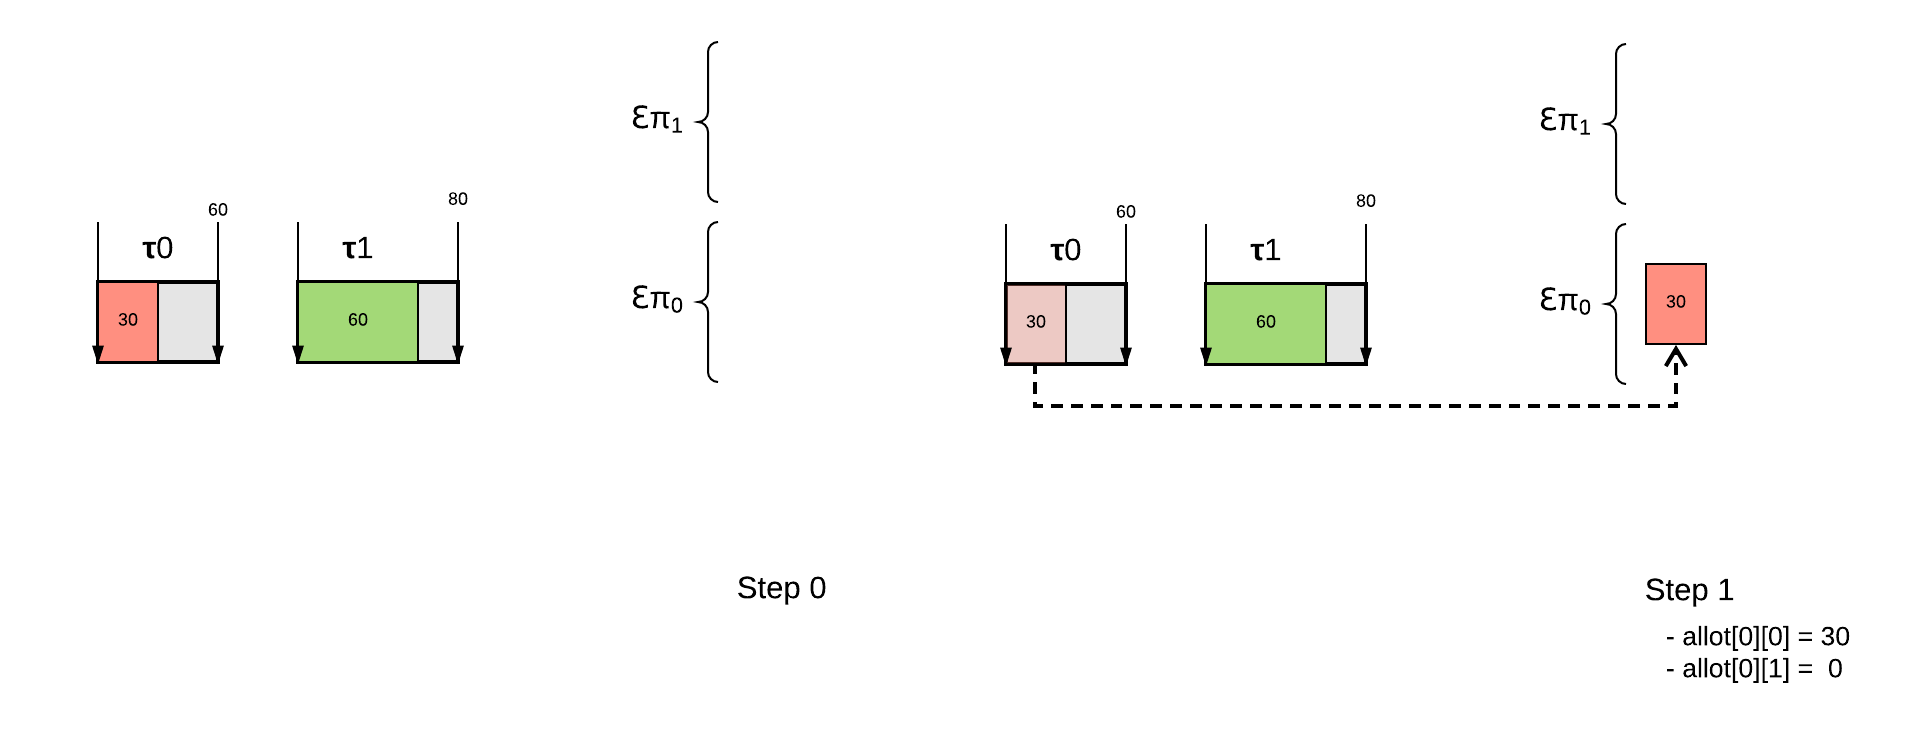
\includegraphics[scale=1]{img/uedf/uedf12}
		\caption{étapes 0 et 1}
		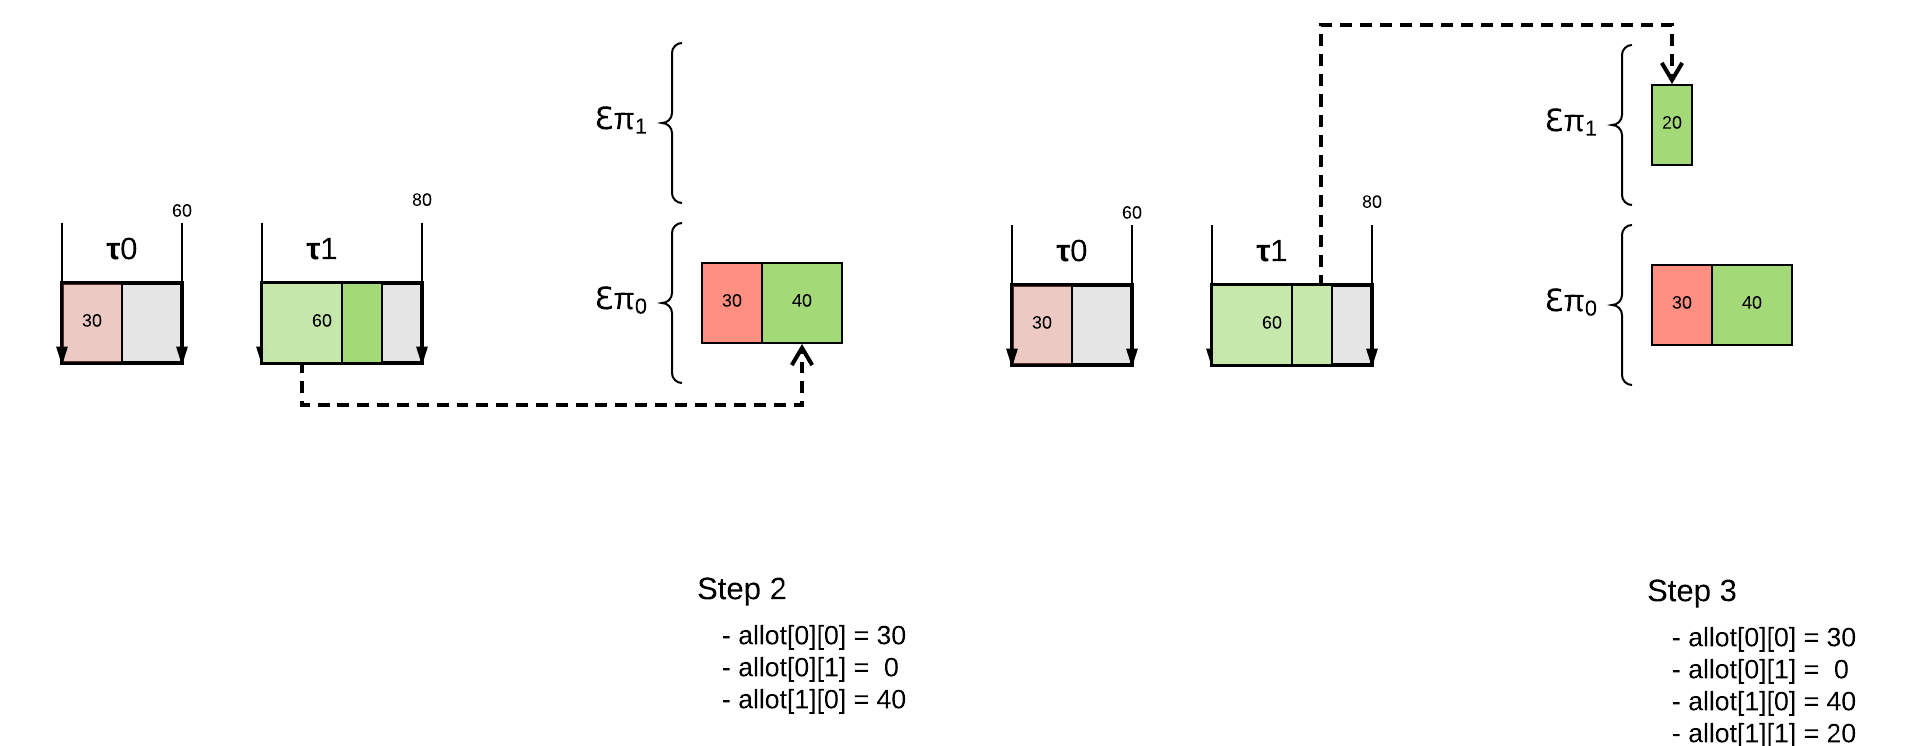
\includegraphics[scale=1]{img/uedf/uedf34}
		\caption{étapes 2 et 3}
	\end{figure}
	\paragraph{Eligible}
	À ce stade, aucune décision d'ordonnancement n'est encore prise, mais des ensembles de tâches (\textit{Eligible}, 
	noté $\epsilon$ dans la suite) sont créés sous forme de listes. Chaque liste \textit{Eligible} définit 
	les seules tâches que les processeurs associés peuvent exécuter (en cela, cette phase d'\textbf{UEDF} peut 
	être considérée comme une phase de partitionnement) durant l'exécution à venir.\newline
	
	Notons que les calculs fournis par l'algorithme permettent en théorie de "remplir" 
	la charge d'un processeur à 100\% d'utilisation avant de passer au suivant. Concrètement, 
	cela signifie que si une tâche a une utilisation de moins de 100\%, elle sera suivie par 
	au moins une partie d'une autre.\newline

	\paragraph{Prise de décision}
	La phase de décision de l'ordonnancement se déroule lors de la phase suivante.
	\textbf{UEDF} s'inspire pour finir de \textbf{EDF-Delay}. 
	Cet algorithme est très simple :
	\begin{itemize}
		\item Une tâche $\tau_i \in \epsilon_j$ est attribuée à un processeur si aucun autre processeur d'index plus bas n'est en train de l'exécuter
		\item $\tau_i$ s'exécute sur le processeur tant qu'$allot_{ij} > 0$.
	\end{itemize}
	
	Nous devons déjà formuler ici une grande nuance par rapport à la faisabilité exacte de cet algorithme. 
	En théorie, l'on est capable de connaître la valeur exacte d'$allot_{ij}$ au temps $t$. En pratique, 
	un système d'exploitation ne permet pas forcément cela, nous en reparlerons ultérieurement.	\newpage
	
	
	\subsection{Comparaison avec Globa-EDF}
	
	Nous avons choisi de comparer \textbf{UEDF} à \textbf{Global-EDF}. La raison de ce choix est simple : 
	cet algorithme est implémenté sur le RTOS HIPPEROS. 
	
	Mais ces deux algorithmes ont de grandes divergences, notamment Global-EDF 
	ne permet pas -- même théoriquement -- d'atteindre l'optimalité. Ceci s'explique par le fait que 
	Global-EDF peut être considéré comme "vertical" là où UEDF serait "horizontal". 
	
		\subsubsection{Fonctionnement très général de Global EDF}
		Afin de montrer la particularité d'\textbf{UEDF}, nous commençons par rappeler le fonctionnement 
		d'un ordonnanceur bien connu et que l'on peut considérer comme "vertical" : \hyperref[GlobalEDF]{Global EDF}\ref*{GlobalEDF}.
		
		L'algorithme est extrêmement simple, et pour les besoins de la comparaison, nous rappelons 
		ici son fonctionnement de façon très résumée.\\
		À un moment \textit{t}, l'ordonnanceur prend sa décision de cette façon :
		si un processeur est libre, il se voit attribué le travail de priorité supérieure parmi 
		tous les travaux actifs. Cela permet d'avoir un algorithme simple et peu gourmand :\newline
		
		On conserve une structure de données 
		ordonnée, comme un \textbf{Heap} \todo{glossaire} qui contient tous les travaux
		devant être exécutés. À chaque fois que l'ordonnanceur doit prendre 
		une décision, il lui suffit de prendre le travail de priorité supérieure et 
		de l'exécuter sur le processeur libre.
		
		L'algorithme ne calcule rien à propos de l'avenir, sa décision au moment \textit{t}
		n'est prise qu'en considérant les travaux à exécuter et la liberté d'un 
		processeur. Il se peut qu'un autre ordonnancement plus efficace 
		réussisse à ordonnancer un système que \textbf{Global EDF} ne puisse pas résoudre...
		Cela rend tout de même l'ordonnanceur "efficace" en terme de calculs, 
		puisqu'il comporte un Heap, de complexité $O(n\log n)$, qui sera mis à jour 
		à chaque changement d'état du travail (relâché -> inséré, 
		exécuté -> retiré du Heap).
		
		En revanche, ce fonctionnement ne permet pas à cet ordonnanceur d'atteindre 
		l'optimalité pour la classe de systèmes périodiques, comme on peut le voir 
		avec cet exemple :
		\todo{montrer un exemple qui rende Global EDF non efficace pour un job}

	
		Nous appelons ce fonctionnement "horizontal" car au lieu de remplir 
		en priorité les processeurs "libres", UEDF va remplir les 
		processeurs par ordre. Ainsi, pour une utilisation inférieure à 100\%, 
		on n'aura besoin que d'un seul processeur. Pour 200, 2 processeurs, bref, 
		pour une utilisation de m * 100 \%, on utilisera m processeurs.
		
		\todo{ajouter une description plus détaillée, avec pseudo code}
		
\section{HIPPEROS}
	\customhighlight{HIPPEROS} (\textbf{HI}gh \textbf{P}erformance \textbf{P}arallel \textbf{E}mbedded \textbf{R}eal-time \textbf{O}perating \textbf{S}ystems)
	est un \customhighlight{RTOS} (Real-Time Operating System) développé depuis plusieurs années par une spinoff de l'ULB.
	Il bénéficie des connaissances apportées par le monde de la recherche dans 
	le domaine des systèmes critiques avec multic\oe{}urs. Une de ses particularités 
	est sa modularité, qui permet d'adapter ses possibilités en fonction du système 
	lors de la compilation de l'OS, ainsi peut-on différencier principalement 
	deux installations en fonction des particularités. 
	
	\customhighlight{HIPPEROS} est un candidat idéal pour l'implémentation d'un ordonnanceur 
	global. Il a cependant un fonctionnement propre qui pourra rendre l'implémentation 
	plus ou moins facile, et poser un certain nombre de problèmes. 
	En résumé, une nouvelle implémentation sur un OS différent 
	peut elle-aussi apporter à la connaissance générale des détails importants.
		

\section{Difficultés liées à l'implémentation}

	Dans cette partie, nous allons analyser les difficultés rencontrées lors de l'implémentation en elle-même, 
	en nous concentrant sur celles liées aux aspects théoriques d'origine. 

	\subsubsection{Accès aux données nécessaires}
	
		Dans \textbf{HIPPEROS}, il existe d'autres ordonnanceurs déjà implémentés. Il convenait donc 
		de s'adapter à l'implémentation existante. Cela signifie des accès parfois compliqués afin d'accéder 
		aux informations de la tâche.\newline
		
		\textbf{HIPPEROS} ordonne les tâches de cette façon : 
		\begin{itemize}
			\item Les données concernant les tâches sont accessibles via un objet \textit{task}. Ces 
			données sont statiques.
			\item Certaines données concernent une autre structure, appelée \textit{process}. L'accès 
			à cette structure ne se fait pas de la même façon. 
			\item Les données concernant le travail sont dans la structure \todo{je saisplus}.
		\end{itemize}
		Une première chose à laquelle il faut être attentif est de rendre possible les accès 
		à ces données, par exemple en conservant des tableaux de références, afin de minimiser les temps 
		d'accès. Cela nécessite de faire un choix : on optimise le temps d'accès en conservant plus de données. \newline
	
		Les autres ordonnanceurs n'utilisent pas vraiment les données concernant le temps 
		d'exécution de la tâche. Pour \textbf{UEDF}, nous avons besoin d'un accès efficace et 
		correctement mis à jour à ces données. Typiquement, le \textbf{Resting Execution Task} est utilisé en plein 
		milieu du calcul \textbf{Allot}, ce qui signifie que lors du calcul, il doit être possible 
		de récupérer ces données. Or, cela n'est pas tout à fait possible, ou du moins, pas idéalement. 
		En fait, \textbf{HIPPEROS} met à jour le temps exécuté d'une tâche lors d'un changement d'état de celle-ci. 
		Ainsi, si un travail est effectué, on note dans ses états le moment auquel il a été dispatché.
		Au temps \textit{t}, si l'on veut savoir combien de temps il a été effectué, s'il n'a pas changé 
		d'état, il faudra calculer ce temps dans \textbf{UEDF} car \textbf{HIPPEROS} n'aura pas encore mis à 
		jour cette donnée.\newline
		Si en terme de temps d'accès, cette requête n'est pas très compliquée, il n'en demeure pas moins 
		que le résultat sera un peu approximatif, puisque l'ordonnanceur n'arrête pas l'exécution des tâches pendant 
		son exécution. Cela ne change pas fondamentalement le calcul car cela change des valeurs très faibles, 
		mais cela constitue une adaptation de la théorie en pratique.\newline
		
		
		Une des critiques que l'on peut adresser à l'algorithme \textbf{UEDF} est sa complexité. 
		Pour rappel, à chaque ajout de travail dans l'ensemble des tâches actives, il faut 
		parcourir la liste entièrement, et ce plusieurs fois, ce qui mène à 
		une complexité de \todo{chercher... $O(m \times n)$ ?}. 
		Certes, avec une astuce, proposée par G. Nelissen dans sa thèse, il est possible de réduire 
		la complexité du calcul, néanmoins pas sa fréquence. Il est donc primordial de réussir à 
		minimiser la complexité, et maximiser l'efficacité des structures de données utilisées par l'algorithme.\newline
		
		
		En théorie, lorsqu'on doit parcourir une liste ordonnée et supprimer des éléments régulièrement, 
		qui ne sont forcément la tête de la liste, le Heap est assez mal adapté. En premier lieu, 
		nous avons donc implémenté une liste liée, laissant à une étape ultérieure l'optimisation. 
		Pour citer cette phrase bien connue de T. Khuhn \todo{citation sur optimisation}.
		
		Ces listes sont connues pour avoir de mauvaises 
		performances, et elles impactaient énormément le temps de calcul d'\textbf{UEDF}. 
		Nous verrons que par la modification de cette structure, nous avons déjà réduit drastiquement 
		le temps d'exécution du calcul. Est-ce suffisant pour permettre à \textbf{UEDF} d'être utilisé dans la réalité est une question à laquelle nous répondrons dans le prochain chapitre.
		
	\subsubsection{Modèle séquentiel}
	
		Le problème que nous venons d'évoquer plus haut concernant le \textbf{RET}. On a besoin de données 
		à un certain moment qui ne sont pas encore disponibles et qu'\textbf{UEDF} doit calculer lui-même. 
		
		Dans l'exposé idéal d'un ordonnanceur, l'exécution s'arrête, l'ordonnanceur fait ses calculs, créé son 
		ordonnancement, et dispatche les travaux selon les règles qui lui sont propres avant que l'exécution reprenne. 
		Un ordonnanceur fait bien souvent partie des tâches lui-même, et il faut qu'il soit lui-même ordonnancé, 
		afin de pouvoir changer l'exécution en cours. Toujours est-il qu'en attendant, l'exécution sur les autres cœurs 
		n'est pas stoppée, et les données continuent d'évoluer. 
		
		Un cas de figure peut se produire, par exemple : au lieu de n'avoir qu'un seul travail à ajouter dans 
		l'ensemble de tâches actives, on peut très bien avoir ajouté plusieurs travaux ainsi que terminé un travail.
		Cela ne change pas fondamentalement le calcul : dans le cas de multiples travaux terminés et pas de travaux nouveaux, 
		il suffit de prendre une décision pour chaque processeur libre (on créé une liste).
		Dans le cas de multiples ajouts de nouveaux travaux, c'est également simple, puisque l'on 
		doit de toute façon recalculer Allot pour tout l'ensemble, on fait la même chose. 
		
		Ce qui est plus compliqué, c'est s'il y a les deux. Mais s'il y a les deux, on doit 
		de toute façon recalculer un nouvel ordonnanceur, donc on obtient ce fonctionnement :
		
		Si un ou des nouveaux travaux : un booléen indique qu'il faut recalculer Allot. Puis, 
		on fait l'assignation ensuite.
		S'il n'y a pas de nouveaux travaux mais qu'il y a un ou des travaux terminés :
		pour chaque processeur libre, prendre une décision pour la suite.\newline
		
		C'est aussi simple que ça, mais cela n'est pas décrit dans le papier et représente une 
		adaptation du modèle.
	
	
		
	\subsubsection{WCET}
		\textbf{UEDF} est assez original par rapport aux autres algorithmes implémentés dans \textbf{HIPPEROS} 
		par rapport à l'utilisation des données. Par exemple, pour le calcul d'\textbf{Allot}, il faut accéder 
		au \textbf{RET} \todo{inclure lien vers RET}, qui dépend du \textbf{WCET}, et du temps déjà exécuté. 
		Le \textbf{WCET}, dans UEDF, est une donnée centrale. Elle est utilisée dans beaucoup de calculs, et 
		son importance est grande pour le résultat. Or, cette donnée n'est pas évidente à produire. \newline
		
		Notre travail nous amène à nous pencher sur ce sujet, qui dépasse largement la portée de ce travail. 
		Néanmoins, voici ce que l'on peut retenir pour nos besoins :\\
		Ce sujet est documenté dans la littérature scientifique. Il n'est pas évident de déterminer le 
		\textbf{WCET} pour toutes les tâches. Mettons qu'une tâche doive faire des lectures/écritures, 
		ce temps-là devra être considéré. Il est possible de déterminer le nombre d'instructions, 
		et donc un temps théorique en fonction de la machine utilisée pour l'exécuter, mais cela dépend 
		parfois de l'exécution. En effet, certaines opérations, en fonction des données, ne vont pas prendre 
		le même temps, or, ce que l'on cherche à déterminer et le pire des cas.\newline
	
		Pour les besoins de ce travail, nous avons simplifié la question, considérant des tâches 
		non dépendantes les unes des autres, avons fait un calcul à la main pour évaluer le 
		nombre d'opérations, et avons vérifié le temps d'exécution des tâches en exécutant un grand nombre 
		de fois les tâches et pris le pire temps comme valeur de \textbf{WCET}. Cela ne garantit en fait 
		pas que le \textbf{WCET} soit réellement le pire des cas, mais cela est suffisant pour nos besoins ici.
	
	\subsubsection{Utilisation instantanée et interruptions}

	L'algorithme d'ordonnancement d'\textbf{UEDF} utilise comme variable l'utilisation instantanée du système. 
	Pour rappel, celle-ci est définie par la somme des utilisations des tâches actives à l'instant $t$, 
	tâche active signifiant tâche ayant relâché un travail qui n'a pas encore atteint son échéance. 
	On considère donc ici pouvoir comptabiliser tous les processus en exécution. Ceci est 
	en fait assez théorique et pose certains problèmes.
	
	Le problème de l'évaluation du \textbf{WCET} posé précédemment, il faut à ce stade rappeler comment 
	fonctionne un système d'exploitation.
	
	D'un point de vue théorique, si l'on estime voir l'ensemble des tâches dans un ensemble uniforme, 
	en pratique, ce n'est pas forcément le cas. Dans ce travail, une partie de la complexité est 
	donc éloignée. NUMA = non-memory-uniform-access
	
	Linux traite chaque processus comme un thread. Les threads ont un domaine. 
	https://lwn.net/Articles/80911/
	https://hal.archives-ouvertes.fr/hal-01295194/document  sur le scheduler linux
	\todo{développer cette partie et sourcer}
	

	L'ordonnanceur n'est pas compté dans les tâches, c'est un module du kernel. Par conséquent, il n'est pas comptabilisé 
	dans l'utilisation instantanée. Il fait partie de ce tas que l'on nomme "overhead" et dans lequel 
	on met tout ce qui prend du temps sans être régulier. 
	Migrations, ordonnanceur, interruptions... Ces temps ne font pas partie du système, mais ils occupent
	pourtant du temps.
	
	Ce n'est pas la seule tâche qui n'est pas comptabilisée dans l'ensemble, puisqu'on peut définir des 
	interruptions côté utilisateur. 
	Concrètement, on imagine une sonde qui envoie très rarement des données. On ne réserve 
	pas de temps, on vérifie régulièrement qu'elle a des données à traiter, et si c'est le cas, on les traite.\\
	C'est un cas d'utilisation du system domain : garantir que les données seront traitées vite, dès qu'elles arrivent, 
	mais ne pas attribuer une tâche pour le faire régulièrement.
	Dans un système d'exploitation, l'ordonnanceur est chargé d'ordonnancer les tâches selon leurs priorités. 
	Pour ce faire, la norme \textbf{POSIX} définit des niveaux de priorité pour les threads. 
	\textbf{HIPPEROS }se base sur la même approche, et définit plusieurs niveaux également. C'est ainsi 
	qu'un thread peut être de scope system, et dans ce cas, sa priorité est haute, ou de priorité 
	moindre, et il sera ordonnancé par \textbf{UEDF}.\newline
	
	Tout ceci montre les limites d'un modèle où l'on charge l'utilisation des processeurs à 100\% avant de 
	passer au suivant. Certes, l'utilisation sera optimisée, dans le sens où l'on 
	pourra utiliser moins de processeurs, mais en revanche, on 
	répartir moins bien la somme de travail, et atteint très vite une somme critique pour les processeurs utilisés.

\section{La vérification de l'implémentation : tests unitaires simulés avec des sets créés}

	Une des difficultés rencontrée lors de l'implémentation d'\textbf{UEDF} a été de s'assurer de la correction de l'algorithme. 
	Aucune autre implémentation n'était accessible sur un autre \textbf{RTOS}, de fait, et donc il n'y avait pas de 
	comparaison possible. En outre, nous trouvons bien un invariant dans la thèse de G. Nelissen, ce qui assure 
	que l'algorithme a bien réservé du temps pour toutes les tâches présentes dans l'ensemble 
	(ce qui doit être vrai pour tout système où $instant\_utilisation <= m$), mais ne garantit pas 
	qu'il n'y a pas d'erreurs ensuite dans la répartition des sous-systèmes, etc. Pour cela, il faut encadrer 
	l'exécution d'autres tests. \newline

	Avant de nous lancer dans l'exécution réelle de l'algorithme, une grande partie du travail a consisté 
	à simuler l'exécution du programme à l'aide de tests unitaires. Ceux-ci ont été pensés de sorte à avoir 
	une couverture relativement élevée du code (50 \% environ) afin d'éviter les surprises lors du passage 
	

\section{Tests globaux}

\subsection{Génération de tâches}

\subsection{Overhead}

\section{Comparaison avec G-EDF}
